\documentclass[12pt]{article}
\usepackage[utf8]{inputenc}
\usepackage[french]{babel}
\usepackage{amsmath,amsthm,amsfonts,amssymb}
\usepackage{lmodern}
\usepackage[top=2.4cm,bottom=2.4cm,left=2cm,right=2cm]{geometry}
\usepackage{hyperref}
\usepackage{multicol}
\usepackage{enumitem}
\usepackage{listings}
\usepackage[dvipsnames]{xcolor}
\usepackage{tikz}
\date{}
\author{MABROUK Fayez}
\title{{\bf  Génie logiciel} \\
	Rendu de Td \no 9  \\
	{\small L3 Informatique appliquée 2022-2023} \\
	{\it \small \no étudiant : 22213839}}
\begin{document}
	\maketitle
	\newpage
	\section{Projet fil rouge}
	Avec le même trinôme que les semaines passées, vous devez commencer la modélisation de votre
	projet. Vous devez modéliser les exigences fonctionnelles (définies en TD de la semaine 3) de votre
	projet sous forme de cas d’utilisation. Les diagrammes devront être rassemblés dans un document.\\
	\\
	Pour chaque cas d’utilisation, vous préciserez l’exigence fonctionnelle à laquelle il répond ; les
	acteurs, vos choix de modélisation éventuels, et un glossaire si nécessaire.\\
	\\
	Pour chaque cas d’utilisation développé, proposez un diagramme de séquence montrant
	l’agencement des interactions.\\
	\\
	En plus de ces diagrammes, vous montrerez (explicitement dans votre rapport) quels objets ont été
	découverts.\\
	\\
	Vous devez modéliser au minimum 5 exigences fonctionnelles.
	\\
	\\
	\textbf{Groupe : PHAN Dao , MABROUK Fayez , AHMED-ZAID Macyl}
	 \\
	 \\
	Énoncé de projet : \\
	Projet 2 – Guide touristique sur smartphone \\
	L’objectif de ce projet est de proposer une application permettant aux touristes de découvrir\\
	Paris. Cette application doit permettre la géolocalisation de l’utilisateur, et proposer des
	activités proches, issues d’une base de données. Des fonctionnalités telles que la création de
	balades selon des critères définis par l’utilisateur ou l’estimation de l’affluence pourront être
	envisagées .\\
	\\
	Les exigences fonctionnelles (TD \no 3):\\
	\begin{itemize}
		\item[* ] Créer un trajet personnalisable grâce à une interface avec ou sans l’intervention de \\l’utilisateur.
		\item[* ] Ajouter des lieux favoris et de les supprimer.
		\item[* ] Partager les balades de l’utilisateur avec d’autres utilisateurs sur une page communautaire.
		\item[* ] Sauvegarder les trajets d’un utilisateur.
		\item[* ] Retrouver les points d’intérêt de la ville de Paris à l’aide d’une base de données.
		\item[* ] Gérer les comptes, de la création, l’identification à l’oubli de ses derniers.
		\item[* ] Interagir avec différents outils sur la carte avec : une description des outils et des lieux populaires,des photos, un outil Zoom+/- et des icônes spécifiques pour les attractions populaires de la ville de Paris.
		\item[* ] Afficher les chemins les plus optimaux avec une api google ou avec un algorithme de calcul de chemin.
		\item[* ] Demander à l’utilisateur d’activer la géolocalisation et de traiter ses données.
		\item[* ] Estimer l’affluence en temps réel.
		\item[* ] Proposer des lieux en fonction de l’affinité de l’utilisateur.
		\item[* ] Fonctionner en ligne et hors ligne (avec moins de 
		fonctionnalités).
		
		
	\end{itemize}

%\newpage
\textbf{\underline{Diagrammes de séquence \& cas d'utilisations}}
\\

\begin{itemize}
	\item[* ]  Partager les balades de l’utilisateur avec d’autres utilisateurs sur une page communautaire.
		\begin{figure}[!hbtp]
			\centering
			\includegraphics[scale=0.65]{Capture1_s.PNG}
			%\caption{Légende de l'image}
		\end{figure}
		\begin{figure}[!hbtp]
		\centering
		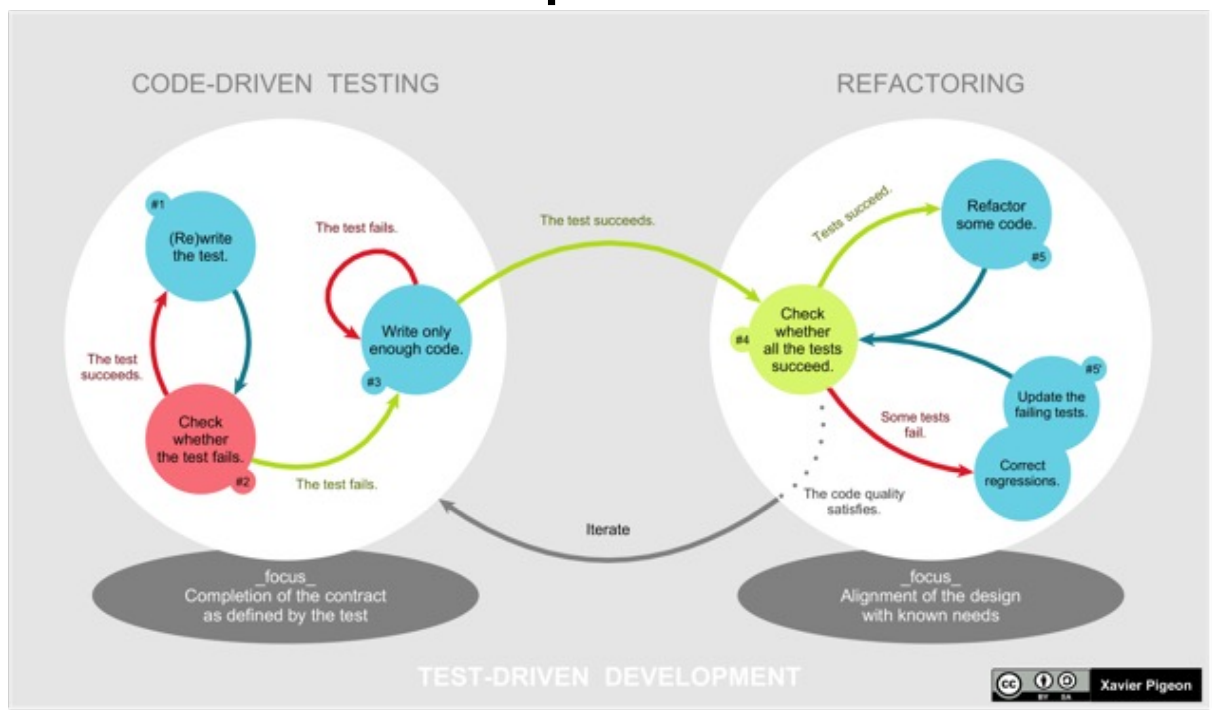
\includegraphics[scale=0.5]{Capture1.PNG}
		%\caption{Légende de l'image}
	\end{figure}
\begin{itemize}
	\item Explications : 
	L'objet interface représente toute la couche avec laquelle interagit l'utilisateur directement, l'objet serveur communauté est apparu pour modéliser toutes les interactions entre les utilisateurs sur le net. Et l'API Carte représente l'API elle-même dans le monde réel.
	
\end{itemize}
\item[* ]  Afficher les chemins les plus optimaux avec une api google ou avec un algorithme de calcul de chemin.
%\newpage
\begin{figure}[!hbtp]
	\centering
	\includegraphics[scale=0.65]{Capture2_s.PNG}
	%\caption{Légende de l'image}
\end{figure}
\begin{figure}[!hbtp]
	\centering
	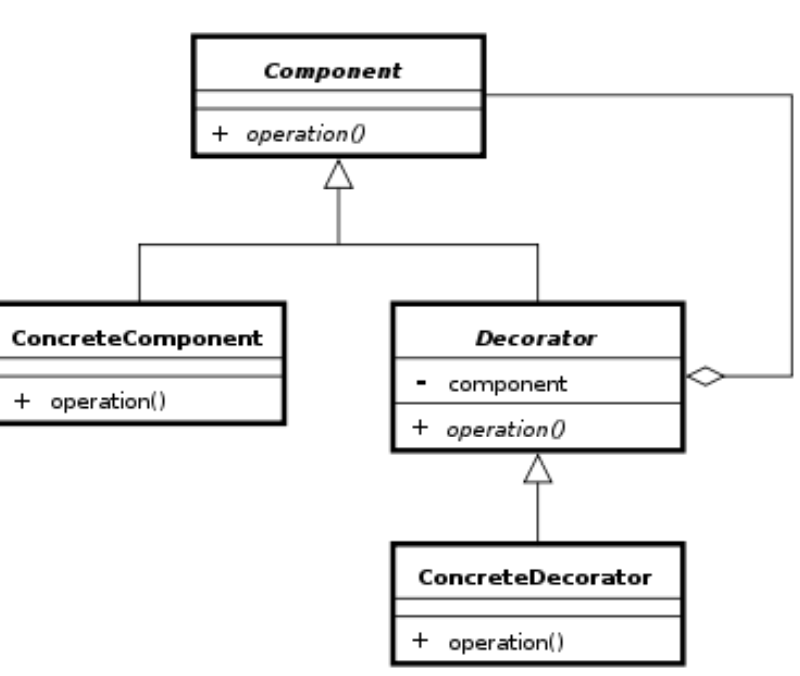
\includegraphics[scale=0.65]{Capture2.PNG}
	%\caption{Légende de l'image}
\end{figure}
\begin{itemize}
	\item  Explications : 
	L'objet interface représente toute la couche avec laquelle interagit l'utilisateur directement, l'objet Gestionnaire de requêtes API pour recevoir les requêtes et les transmet aux Gestionnaire de graphes . Et Gestionnaire de graphes pour appliquer l’algorithme le plus efficace au niveau de réseaux en utilisant API google.
	
\end{itemize}
\end{itemize}
\newpage
\begin{itemize}
	\item[* ] Ajouter des lieux favoris et de les supprimer.
		\begin{itemize}
		\item[(1)] \textbf{Diagramme cas d'utilisation:}
	\begin{figure}[!hbtp]
		\centering
		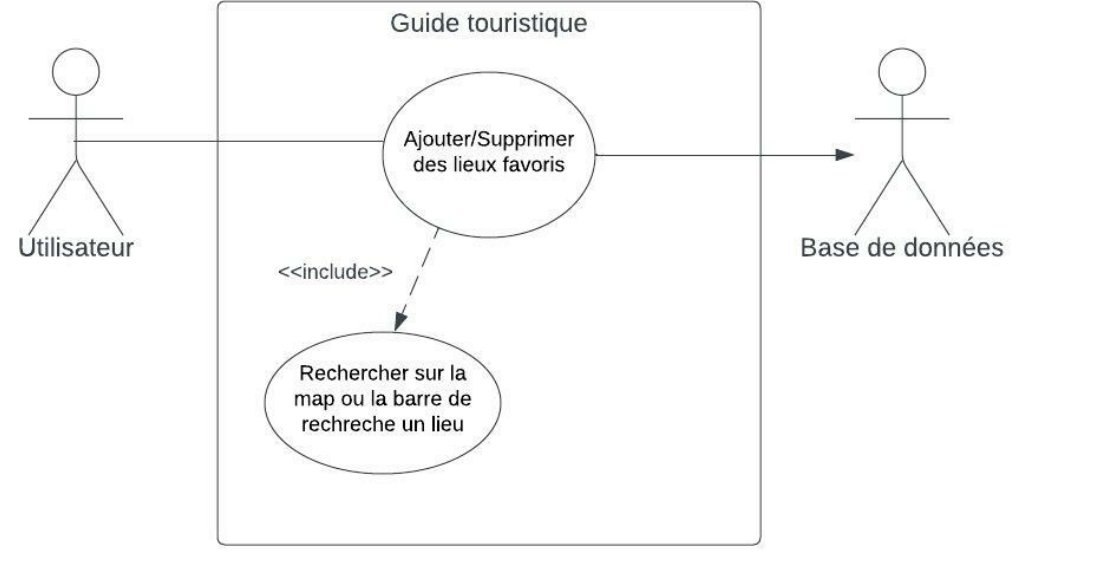
\includegraphics[scale=0.75]{Capture3_s.PNG}
		%\caption{Légende de l'image}
	\end{figure}
\item[(2)] \textbf{Diagramme de séquence:}
\begin{figure}[!hbtp]
	\centering
	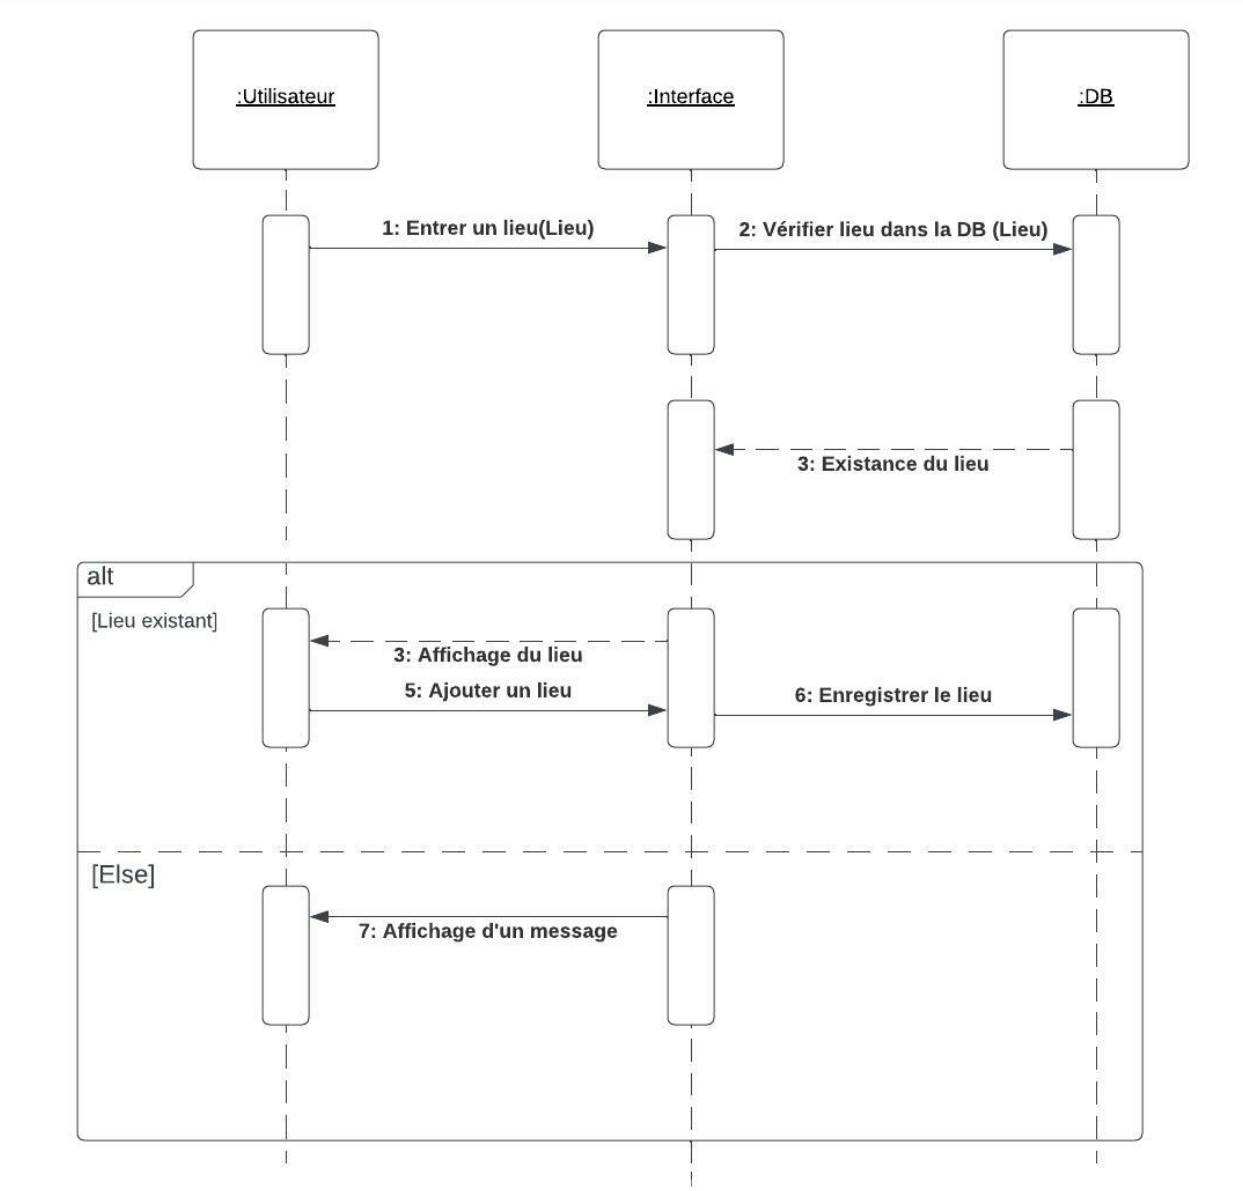
\includegraphics[scale=0.75]{Capture3_2.PNG}
	%\caption{Légende de l'image}
\end{figure}
\end{itemize}
\end{itemize}
\newpage
\begin{itemize}
	\item[* ]  Sauvegarder les trajets d’un utilisateur.
	\begin{itemize}
		\item[(1)] \textbf{Diagramme cas d'utilisation:}
	\begin{figure}[!hbtp]
		\centering
		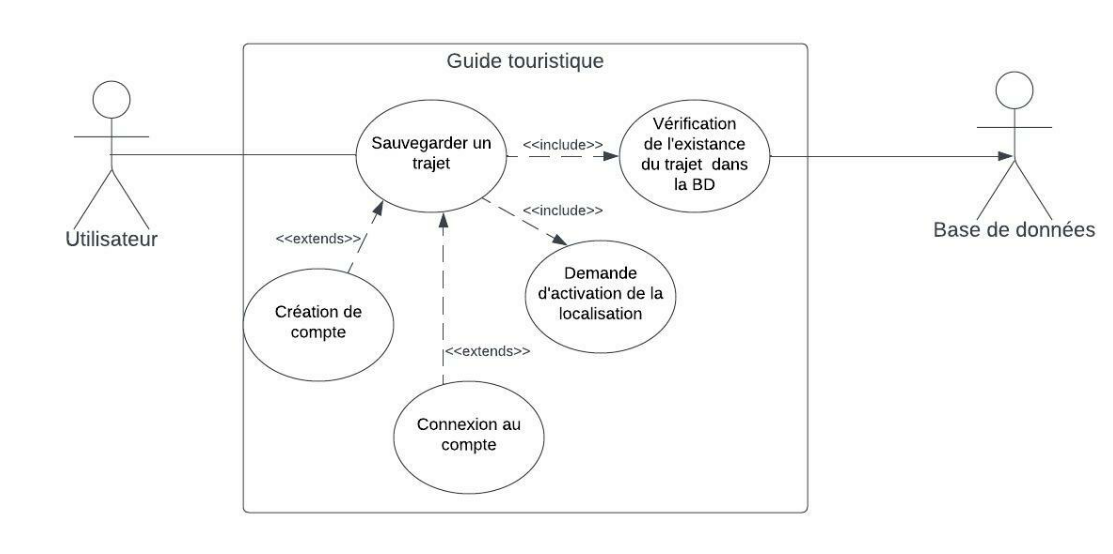
\includegraphics[scale=0.75]{Capture4.PNG}
		%\caption{Légende de l'image}
	\end{figure}
\item[(2)] \textbf{Diagramme de séquence:}
	\begin{figure}[!hbtp]
	\centering
	\includegraphics[scale=0.65]{image1.jpg}
	%\caption{Légende de l'image}
\end{figure}
\end{itemize}
\end{itemize}
\newpage
\begin{itemize}
	\item[* ] Gérer les comptes, de la création, l’identification à l’oubli de ses derniers.
		\begin{itemize}
		\item[(1)] \textbf{Diagramme cas d'utilisation:}
	\begin{figure}[!hbtp]
		\centering
		\includegraphics[scale=0.75]{image2.png}
		%\caption{Légende de l'image}
	\end{figure}
	\begin{itemize}
		\item Explications : On considère qu’un utilisateur peut soit choisir d’essayer de se connecter ou de modifier son mot de passe qu’il aurait oublié.
		Chacune des opérations respectives engendre l’utilisation de la base de donnée pour vérifier ou modifier les valeurs internes.
		L’identification entraîne impérativement une réaction d’un serveur, que ce soit pour autorisé ou refusé l’accès à ce dernier (accès $\Rightarrow$ connexion).
		
	\end{itemize}
\item[(2)] \textbf{Diagramme de séquence:}
\begin{figure}[!hbtp]
	\centering
	\includegraphics[scale=0.75]{image3.png}
	%\caption{Légende de l'image}
\end{figure}
\end{itemize}
\end{itemize}
\newpage
\begin{itemize}
	\item[* ] Proposer des lieux en fonction de l’affinité de l’utilisateur.
	\begin{itemize}
		\item[(1)] \textbf{Diagramme cas d'utilisation:}
	
	\begin{figure}[!hbtp]
		\centering
		\includegraphics[scale=0.75]{image4.png}
		%\caption{Légende de l'image}
	\end{figure}
\begin{itemize}
	\item Ici, un algorithme va vérifier dans la BDD l’historique des lieux les plus fréquentés en fonction d’un thème précis (un thème peut être une période de l’année, un mot clé « Parc » ou encore rien du tout (par défaut on recherche ce que l’utilisateur à le plus visité ces derniers temps)).
	Enfin, le serveur va ensuite proposer à l’utilisateur des lieux non visités par ce dernier parmi la liste des lieux résultant de l’algorithme.
	
\end{itemize}
\item[(2)] \textbf{Diagramme de séquence:}
	\begin{figure}[!hbtp]
	\centering
	\includegraphics[scale=0.75]{image5.png}
	%\caption{Légende de l'image}
\end{figure}
\end{itemize}
\end{itemize}

\end{document}